\section{Integration range over $\omega$}

\begin{figure}[ht!]
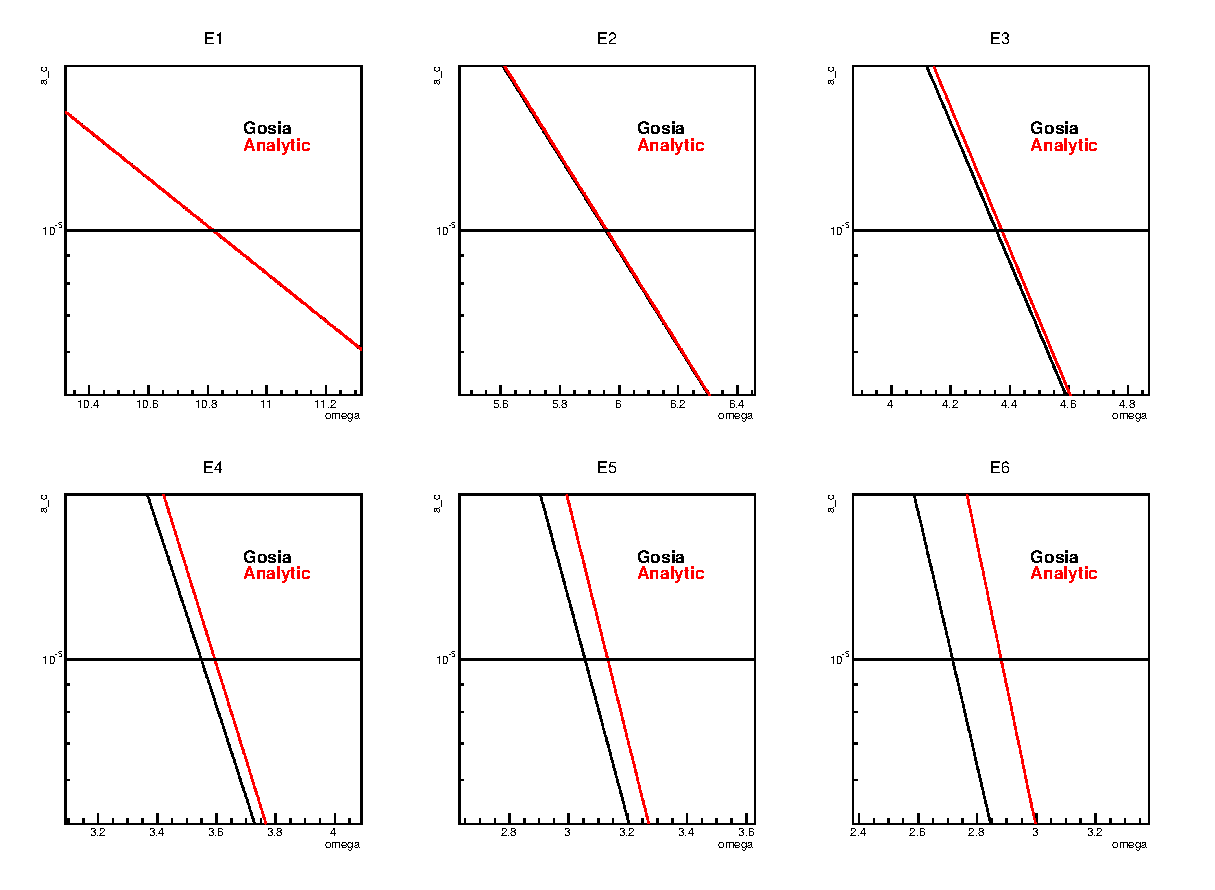
\includegraphics[width=\textwidth]{integration_range.eps}
\caption{Comparison of integration range calculated with Gosia's
formula and with the analytic solutions}
\end{figure}

\noindent We define (c.f. Gosia manual Eq. 6.1):

\begin{equation}
a_c = {1 \over 4} {
\displaystyle \int_{-\infty}^\infty Q_{\lambda 0}(\epsilon = 1, \omega) d\omega
- \displaystyle \int_{-\omega_{max}}^{\omega_{max}} Q_{\lambda 0}(\epsilon = 1, \omega) d\omega
\over
\displaystyle \int_{-\infty}^\infty Q_{\lambda 0}(\epsilon = 1, \omega) d\omega
}
\end{equation}

\subsection{E1}

\noindent Taking the formula for Q from the manual and substituting
$\epsilon$ = 1 we get:

\begin{equation}
Q_{\lambda 0}(\epsilon = 1, \omega) = {1 \over 2}{1 \over \cosh(\omega)
+ 1}
\end{equation}

\noindent Using the relation:

\begin{equation}
{\displaystyle \int_{-\omega_{max}}^{\omega_{max}} Q_{\lambda
0}(\epsilon = 1, \omega) d\omega} =
\tanh{\omega \over 2}
\end{equation}

\noindent So:

\begin{equation}
a_c = {1 \over 4}(1 - \tanh{\omega \over 2})
\end{equation}

\noindent And using:

\begin{equation}
\textrm{arctanh}~ x = {1 \over 2} \ln\big({1 + x \over 1 - x}\big)
\end{equation}

\noindent we have:

\begin{equation}
\omega = \ln \big({1 - 2 a_c \over 2 a_c}\big)
\end{equation}

\noindent This is not what Gosia uses, but for small $a_c$, we can
neglect a term:

\begin{eqnarray}
\omega &=& \ln \big({1 \over 2 a_c}\big)\nonumber\\
&=& -\ln 2 - \ln a_c
\end{eqnarray}

\noindent which is what Gosia has.

\subsection{E2}

\noindent In a similar manner we get:

\begin{equation}
a_c = {1 \over 4} \big[1 - \big({\sinh(\omega) (\cosh(\omega) + 2) \over
(\cosh(\omega) + 1)^2}\big)\big]
\end{equation}

\subsection{E3}

\begin{equation}
a_c = {1 \over4} \big[1 - {1 \over 2}\big({\sinh(\omega) (6 \cosh(\omega) +
\cosh(2\omega) + 8 \over (\cosh(\omega) + 1)^3} \big)\big]
\end{equation}

\subsection{E4}

\begin{equation}
a_c = {1 \over 4} \big[1 - {56 \sinh(\omega) + 28\sinh(2\omega) + 8
\sinh(3\omega) + \sinh(4\omega) \over
8 (\cosh(\omega) + 1)^4}\big]
\end{equation}

\subsection{E5}

\begin{equation}
a_c = {1 \over 4} \big[1 - {
\sinh(\omega)(130 \cosh(\omega) + 46 \cosh(2\omega) + 10
\cosh(3\omega) + \cosh(4\omega) + 128) 
\over
8 (\cosh(\omega) + 1)^5}\big]
\end{equation}

\subsection{E6}

\begin{equation}
a_c = {1 \over 4} \big[1 - {
792\sinh(\omega)+495\sinh(2\omega)+220\sinh(3\omega)+66\sinh(4\omega)+12\sinh(5\omega)+\sinh(6\omega)
\over
32 (\cosh(\omega) + 1)^6}\big]
\end{equation}

